%Ich bin ein TeX Dokument
\documentclass{scrartcl} % KOMA-Script Dokumentenklasse Article
%Für Positionierung von Gleitumgebungen
\usepackage{scrhack}
% Warnung, falls noch einmal kompiliert werden muss
\usepackage[aux]{rerunfilecheck}
% Paket für Schriftarteinstellung, muss immer geladen werden
\usepackage{fontspec}
% Deutsche Spracheinstellungen, wichtig z. B. für korrekte Trennung
\usepackage[ngerman]{babel}
% mehr Pakete hier
\usepackage{amsmath}
\usepackage{amssymb}
\usepackage{mathtools}
%ISO Normen benutzen
\usepackage[
math-style=ISO,
bold-style=ISO,
sans-style=italic,
nabla=upright,
partial=upright,
]{unicode-math}
%Für korrekte Zahlen mit Einheiten
\usepackage[
locale=DE,
separate-uncertainty=true,
per-mode=symbol-or-fraction,
]{siunitx}
% Unterstützung für Links und PDF Metadaten
\usepackage[unicode]{hyperref}
\usepackage{bookmark}
%Für das Einbinden von Grafiken
\usepackage{graphicx}
%Positionierung von Gleitumgebungen
\usepackage{float}
% Einstellungen hier, z.B. Fonts
\setmathfont{Latin Modern Math}
\floatplacement{figure}{H}
\floatplacement{table}{H}
\begin{document}
\title{Titel}
\author{Henry Krämerkämper \and Christopher Breitfeld}
\date{29.10.2020}
\maketitle
\newpage
\tableofcontents
\newpage
\section{Einleitung}
Der Versuch "Die Wärmepumpe", welcher im folgenden erklärt und durchgeführt wird, behandelt den Transport von
Wärmeenergie von einem kälteren zu einem wärmeren Reservoire. Nach dem zweiten Hauptsatz der Thermodynamik sind beide
Flussrichtungen möglich, nur ist für den Transport vom kälteren zum wärmeren Reservoir zusätzliche Arbeit nötig. Diese verrichtet die Wärmepumpe.
Im folgenden werden Merkmale dieser behandelt, in etwa die Güteziffer der Pumpe sowie ihr Massendurchsatz und der Wirkungsgrad des Kompressors.
\section{Theoretische Grundlagen}
  \subsection{Die Güteziffer}
  Die hier verwendete Wärmepumpe wird unter anderem charakterisiert durch die Güteziffer $ v $. Sie gibt das Verhältnis zwischen der aufgewendeten Arbeit für den Wärmetransport
  $ A $ und der transportierten Wärmeenergie $ Q_\text{transp} $ an. Eine Formel für die Berechnung der Güteziffer lässt sich wie folgt herleiten: \\
  \\
  Wir bezeichnen die den wärmeren Reservoire 1 zugeführte Wärmeenergie als $ Q_\text{1} $ sowie die dem kälteren Reservoire 2 entnommene Wärmeenergie als $ Q_\text{2} $.
  Dann gilt nach dem ersten Hauptsatz der Thermodynamik
  \begin{equation}
    Q_\text{1} = Q_\text{2} + A.
    \label{eqn:wärmeenergie1}
  \end{equation}
  Dann ist das Verhältnis zwischen transportierter Wärmeenergie und aufgewendeter Arbeit
  \begin{equation}
    \frac{Q_\text{1}}{A} = v.
    \label{eqn:güteziffer}
  \end{equation}
  Um die Güteziffer einer idealen Wärmepumpe zu berechnen, betrachten wir die Zusammenhänge nach dem zweiten Hauptsatz der Thermodynamik:
  %Finde ich persönlich schwach formuliert, hier müsste nochmal nachgearbeitet werden
  \begin{equation}
    \frac{Q_\text{1}}{T_\text{1}} - \frac{Q_\text{2}}{T_\text{2}} = 0
    \label{eqn:wärmeenergie2}
  \end{equation}
  Gleichung \eqref{eqn:wärmeenergie2} gilt nur unter der Vorraussetzung, dass der Prozess reversibel abläuft.
  Da dies in der Realität nicht möglich ist, muss \eqref{eqn:wärmeenergie2} im Falle eines irreversiblen Prozesses
  anders formuliert werden:
  \begin{equation}
  	\frac{Q_\text{1}}{T_\text{1}} - \frac{Q_\text{2}}{T_\text{2}} > 0
  	\label{eqn:wärmeenergie3}		
  \end{equation}
	Aus Gleichung \eqref{eqn:wärmeenergie1} und Gleichung \eqref{eqn:wärmeenergie3} sowie der Definition der Güteziffer 
	\eqref{eqn:güteziffer} ergibt sich die Güteziffer einer idealen Wärmepumpe zu
	\begin{equation}
		v_\text{ideal} = \frac{Q_\text{1}}{A} = \frac{T_\text{1}}{T_\text{1} - T_\text{2}}
		\label{eqn:idealegüteziffer}
	\end{equation}
	Dann gilt analog zu \eqref{eqn:idealegüteziffer} für die reale Güteziffer:
	\begin{equation}
		v_\text{real} < \frac{T_\text{1}}{T_\text{1}-T_\text{2}}
		\label{eqn:realegüteziffer}
	\end{equation}
	An \eqref{eqn:idealegüteziffer} und \eqref{eqn:realegüteziffer} kann man ablesen, dass eine Wärmepumpe eine höhere Güte hat,
	wenn der Temperaturunterschied zwischen Reservoire 1 und Reservoire 2 möglichst gering ist. Das bedeutet, dass der Arbeitsaufwand 
	für geringe Temperaturunterschiede am kleinsten ist.
	%Zeile 95 vielleicht ein bisschen renundant
	\subsection{Der Massendurchsatz}
	Der Massendurchsatz einer Wärmepumpe beschreibt, wieviel Wärme aus dem kälteren Reservoire 2 pro Zeiteinheit entnommen wird. \\
	Mitlhilfe des gemessenen Differenzenquotienten $ \frac{\increment T_\text{2}}{\increment t}$ sowie der Wärmekapazität von Reservoire 2
	$m_\text{2}c_\text{w}$ und der Wärmekapazität der Kupferschlange und des Eimers $m_\text{k}c_\text{k}$ ergibt sich der Massendurchsatz
	zu
	\begin{equation}
		\frac{\increment Q_\text{2}}{\increment t} = (m_\text{2} c_\text{w} + m_\text{k} c_\text{k}) \frac{\increment T_\text{2}}{t}.
		\label{eqn:massendurchsatz1}
	\end{equation}
	Da der Wärmetransport über Verdampfung eines Mediums stattfindet, kann man \eqref{eqn:massendurchsatz1} auch mithilfe der 
	Verdampfungswärme $L$ schreiben:
	\begin{equation}
		\frac{\increment Q_\text{2}}{\increment t = L \cdot \frac{\increment m}{\increment t}
		\label{eqn:massendurchsatz2}	
	\end{equation}

  
\section{Aufgabenteil a)}
  Man stelle die gemessenen Temperaturverläufe in einem geeigneten Diagramm dar. \\
  \\
  Im folgenden Diagramm werden die Verläufe der Temperaturen T1 und T2 in Abhängigkeit der Zeit aufgetragen.
  Alle Werte wurden in SI-Einheiten konvertiert.
  \\
  \begin{figure}
    \centering
    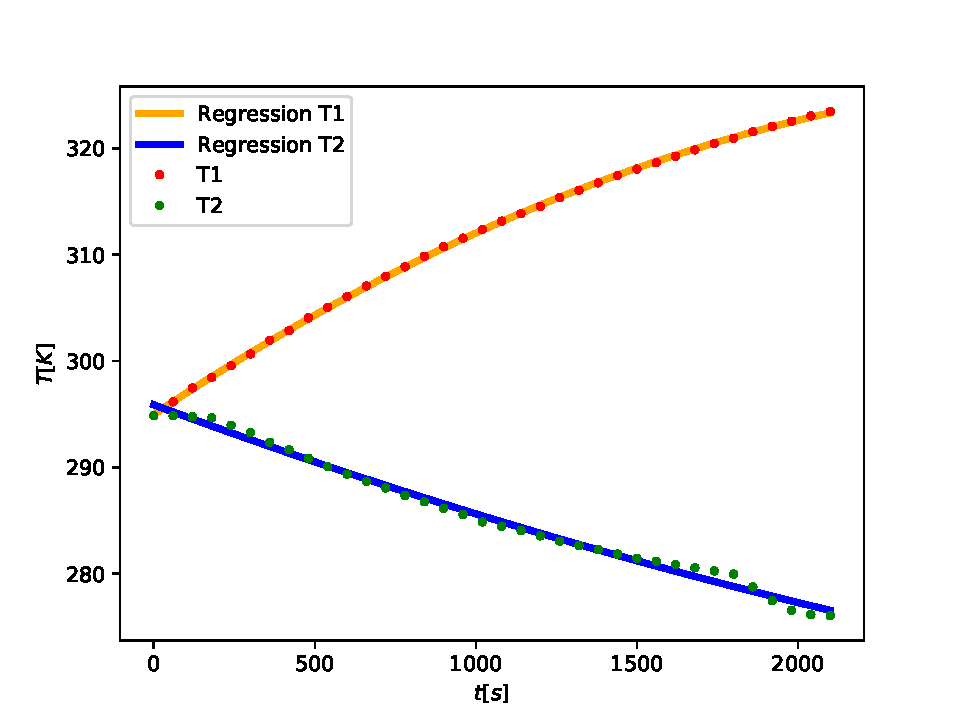
\includegraphics[scale = 0.75]{Temperaturverlaeufe.pdf}
    \caption{Die beiden Temperaturverläufe der Reservoire 1 und 2.}
    \label{fig:TemperaturverlaufA}
  \end{figure}
\section{Aufgabenteil b)}
  Man versuche mit Hilfe einer nicht-linearen Ausgleichsrechnung die gemessenen Temperaturverläufe durch einfache Gleichungen zu approximieren.
  \\
  Die Ausgleichsgleichungen sind ebenfalls in \ref{fig:TemperaturverlaufA} skizziert. Der gewählte Ansatz ist
  \begin{equation}
    T(t) = \symup{A} \cdot t^2 + \symup{B} \cdot t + \symup{C}.
    \label{eq:Regressionsgleichung}
  \end{equation}
  Hierbei ist
\end{document}
